% === Cours de Java
% === Fichier principal
\usepackage{java}

\title{Le Langage Java}
\subtitle{1�re ann\'ee}
\institute[HEB-ESI]{Haute �cole de Bruxelles --- �cole Sup�rieure d'Informatique}    
\date[2011 --- 2012]{Ann�e acad�mique 2011 / 2012}
\author[]{ \small
  M.~Bastreghi \and J.~Beleho \and P.~Bettens \and M.~Codutti 
  \and A.~Hallal \and C.~Leruste \and D.~Nabet \and N.~Pettiaux \and A.~Rousseau
}

\begin{document}
\begin{frame}
\titlepage
\end{frame}

% ===== Inclusion des diffrents chapitres =====
\include{toc}

% ===== Premier quadrimestre
\include{chapitre-contrat}
\include{chapitre-programme}
\include{chapitre-java}
\include{chapitre-jvm}
\include{chapitre-survol-seq}
\include{chapitre-humain}
\include{chapitre-survol-alternative}
\include{chapitre-gram}
\include{chapitre-lex}
\include{chapitre-lisibilite}
\include{chapitre-survol-module}
\include{chapitre-package}
\include{chapitre-survol-boucle}
\include{chapitre-erreur}
\include{chapitre-data}
\include{chapitre-survol-tab}
\include{chapitre-javadoc}
\include{chapitre-tests}
\include{chapitre-var}
\include{chapitre-expr}  
\include{chapitre-assignation} 
\include{chapitre-instr}
\include{chapitre-tableau}

% ====== Second quadrimestre
%=== Cours de Java
%=== Chapitre : OO

\section{L'orient� objet}

\begin{frame}
\begin{block}{\center Le�on \thesection\ ---   \insertsection}
  {
  \begin{multicols}{2}
  \tableofcontents[sectionstyle=hide,subsectionstyle=show/show/hide]
  \end{multicols}
  \bigskip
  }
\end{block}
\end{frame}

\begin{frame}{Avertissement}
Pour qu'un langage soit \textit{orient� objet} il doit poss�der 3 propri�t�s
  \begin{itemize}
  \item L' \emph{encapsulation}
  \item L' \emph{h�ritage}
  \item Le \emph{polymorphisme}
  \end{itemize} 
\bigskip
Trop pour le cours de 1�re ann�e
  \begin{itemize}
  \item Nous allons surtout voir l'encapsulation \\(comme au cours de logique)
  \item Et effleurer le reste $\longrightarrow$ parfois impr�cis
  \end{itemize}
\end{frame}

\begin{frame}{Rappels}
Voici ce que vous avez d�j� vu en logique
\begin{center}
\includegraphics[scale=.6]{../img/oo-rappels}
\end{center}
\end{frame}

\begin{frame}{Pr�sentation de l'exemple}
Illustrons ces concepts avec la notion d'\textit{�tudiant � l'ESI}
\begin{itemize}
 \item Un �tudiant
    \begin{itemize}
    \item poss�de un nom et un num�ro unique
    \item est inscrit dans une ann�e d'�tude
    \item est doubleur ou pas
    \item est un \textit{ancien} (a termin�) ou pas
    \end{itemize}
  \item Il peut r�ussir son ann�e ou la rater
  \end{itemize}
\end{frame}

\subsection{La classe}

\begin{frame}{La classe}
  \emph{Exemple}: Repr�sentation graphique (UML) de la classe \textit{Etudiant}
  \begin{center}
  \begin{tabular}{cl}
    {\small\fcolorbox{black}{bleu}{
      \begin{tabular}{l}
        ~~~~~~~~~Etudiant\\ 
        \hline
        - num�ro : Entier\\
        - nom : Chaine\\
        - ann�e�tude : Entier\\
        - doubleur : Bool�en\\
        - ancien : Bool�en\\
        \hline
        + aR�ussi()\\
        + aRat�()\\
      \end{tabular}
    }} &
    {\small
      \begin{tabular}{l}
        \textbf{Nom de la classe} \\ 
        \textbf{Attributs} \\
        Le "-" indique qu'ils sont \textbf{priv�s}\\
        Connus uniquement dans la classe\\
        En \sigle{Java} on �crira \java|private|\\
        \\
        \textbf{M�thodes}\\
        Le "+" car elles sont \textbf{publiques}\\
        En \sigle{Java} on �crira \java|public|\\
      \end{tabular}
    } \\
  \end{tabular}
  \end{center}
\end{frame}

\subsection{Les objets}

\begin{frame}{Les objets}
  \emph{Exemple} : Repr�sentation graphique de 2 objets (instances) possibles :
  \medskip
  \begin{center}
  \begin{tabular}{cc}
  {\small\fcolorbox{black}{bleu}{
    \begin{tabular}{l}
      \underline{James Gosling}: Etudiant\\ 
      \hline
      - num�ro = 34000\\
      - nom = "James Gosling"\\
      - ann�e�tude = 1\\
      - doubleur = faux\\
      - ancien = faux\\
      \hline
      + aR�ussi()\\
      + aRat�()\\
    \end{tabular}
  }} &
  {\small\fcolorbox{black}{bleu}{
    \begin{tabular}{l}
      \underline{Ada Lovelace}: Etudiant\\ 
      \hline
      - num�ro = 33800\\
      - nom = "Ada Lovelace"\\
      - ann�e�tude = 2\\
      - doubleur = faux\\
      - ancien = faux\\
      \hline
      + aR�ussi()\\
      + aRat�()\\
    \end{tabular}
  }} \\
  \end{tabular}
  \end{center}
\end{frame}

\subsection{Les membres}

\begin{frame}{Les membres}
Chaque instance poss�de les m�mes attributs mais avec des \emph{valeurs diff�rentes}
\\\bigskip
Les m�thodes d'une instance agissent sur les attributs de cette instance 
  \begin{itemize}
   \item La m�thode \textit{aRat�()} d'un �tudiant va mettre \emph{son} attribut \textit{doubleur} � vrai
   \item Que ferait la m�thode \textit{aR�ussi()} ?
  \end{itemize}
\end{frame}

\begin{frame}[fragile]{La classe en Java}
  � ce stade la classe \texttt{Etudiant} peut s'�crire :
  \begin{multicols}{2}  
  \begin{Java}
  public class Etudiant {

    private int num�ro; 
    private String nom;
    private int ann�e�tude;
    private boolean doubleur;
    private boolean ancien; 

    public void aRat�() {
      doubleur = true;
    }
  \end{Java}
  \begin{Java}

    public void aR�ussi() {
      doubleur = false;
      ann�e�tude++;
      if (ann�e�tude == 4 ) {
        ancien = true;
      }
    }

  }  
  \end{Java}
  \end{multicols}
\begin{itemize}
\item Remarquez l'absence de \java{static} pour les m�thodes
\end{itemize}
\end{frame}

\begin{frame}{OO or not OO ?}
On utilisait d�j� \java|class|. On faisait de l'objet ?
\\\bigskip
Oui et non ;)
\begin{itemize}
\item \sigle{Java} est un langage orient� objet
\item Mais il permet une �criture non OO
\item Via l'utilisation de \java|static|
(qui a un sens plus large que nous d�taillerons plus loin)
\end{itemize}
\end{frame}

\begin{frame}{OO or not OO ?}
En gros, on a 2 sortes de classes : 
\\\bigskip
\begin{small}
\begin{tabular}{l|l|l}
\hline\hline
& {\small \emph{approche non OO}} & {\small \emph{approche OO}} \\\hline
But & regrouper des m�thodes & d�finir un type de donn�es \\
Attribut & non (sauf constantes) & oui \\
Instances & non & oui \\
Utilisation via & le nom de la classe & une instance \\
\java|static| & oui & non \\
Fr�quence & rare & fr�quent \\
Exemples & \java|Math| & \java|String|, \java|Scanner| \\
\hline\hline
\end{tabular}
\end{small}
\\\bigskip
\textit{En pratique, on rencontrera des situations mixtes}
\end{frame}

\begin{frame}{Visibilit� des membres}
En \sigle{Java} : 4 visibilit�s
\begin{description}
  \item[public] : visible dans \textbf{toutes} les classes (\java|public|)
  \item[priv�] : n'est accessible que de \textbf{la} classe (\java|private|)
  \item[<<paquet�>>] : visible dans toutes les classes du \textit{package} (pas de mot cl�)
  \item[prot�g�] : pas vu en 1�re ann�e (\java|protected|)
\end{description}
\bigskip
Rappel \emph{bonne pratique} :
\\attributs priv�s / m�thodes publiques
\end{frame}

\subsection{Constructeur}

\begin{frame}[fragile]{Constructeur}
\emph{Exemple} : D�finition d'un constructeur
  \begin{Java}
  public Etudiant (int unNum�ro, String unNom) {
    num�ro = unNum�ro;
    nom = unNom;
    ann�e�tude = 1;
    doubleur = false;
    ancien = false;
  }
  \end{Java}
  Ressemble � une m�thode mais
  \begin{itemize}
    \item Pas de type de retour d�clar�
%    \item En pratique, retourne la r�f�rence de l'objet 
    \item A le m�me nom que celui de la classe
  \end{itemize}
\end{frame}

\subsection{Instanciation}

\begin{frame}[fragile]{Instanciation}
Pour instancier 
\begin{itemize}
\item On utilise l'op�rateur \java|new|
\item On fournit les param�tres au constructeur
\end{itemize}
\medskip
\emph{Exemple} : instanciation d'un �tudiant
\begin{itemize}
\item[]
\begin{Java}
Etudiant ada = new Etudiant(33800, "Ada Lovelace");
\end{Java}
\item Cr�e un nouvel objet \java|Etudiant|
\item Appelle le constructeur pour l'initialiser
\end{itemize}
\end{frame}

\begin{frame}[fragile]{Instanciation}
Une classe est un type \emph{r�f�rence} (comme les tableaux)
\medskip
\\\emph{Exemple} :
\begin{Java}
    Etudiant ada;  // r�f�rence cr��e sur la pile
\end{Java}
\vspace{-10pt}
\begin{center}\includegraphics[scale=.4]{../img/java-oo-alloc1}\end{center}
\begin{Java}
    ada = new Etudiant(33800,"Ada Lovelace"); // objet cr�� sur le tas
\end{Java}
\vspace{-10pt}
\begin{center}\includegraphics[scale=.5]{../img/java-oo-alloc2}\end{center}
\end{frame}

\begin{frame}[fragile]{Appel d'une m�thode}
Utilisation de la notation \textit{point�e} (op�rateur \code{.})
\\\bigskip
\emph{Exemple}
\begin{Java}
public static void main(String[] args) {
    Etudiant ada = new Etudiant(33800, "Ada Lovelace");
    ada.aR�ussi();
}
\end{Java}
\bigskip
Code que l'on peut trouver
\begin{itemize}
\item dans une autre classe
\item dans la classe m�me
\end{itemize}
\end{frame}

\subsection{Accesseurs}

\begin{frame}[fragile]{Accesseurs}
\emph{Accesseur} : m�thode donnant la valeur d'un attribut 
\\\bigskip
\emph{Exemple} : pour notre classe �tudiant
\begin{Java}
  public int getNum�ro() {return num�ro;}
  public String getNom() {return nom;}
  public int getAnn�e�tude() {return ann�e�tude;}
  public boolean isDoubleur() {return doubleur;}
  public boolean isAncien() {return ancien;}
\end{Java}
\bigskip
Par convention, l'accesseur de \java|attribut| est \java|getAttribut| 
(\java|isAttribut| pour un bool�en)
\end{frame}

\begin{frame}[fragile]{Appel d'une m�thode}
\emph{Exemple} : Utilisation des accesseurs
\begin{Java}
public static void main(String[] args) {
    Etudiant ada = new Etudiant(33800, "Ada Lovelace");
    System.out.println(ada.getAnn�e�tude()); // 1
    ada.aR�ussi();
    System.out.println(ada.getAnn�e�tude()); // 2
    System.out.println(ada.isDoubleur()); // false
    ada.aRat�();
    System.out.println(ada.getAnn�e�tude()); // 2
    System.out.println(ada.isDoubleur()); // true
}
\end{Java}
\end{frame}

\subsection{Mutateurs}

\begin{frame}[fragile]{Mutateurs}
\emph{Mutateur} : sert � modifier un attribut 
\\\bigskip
\emph{Exemple} : un mutateur possible pour \textit{Etudiant}
\begin{Java}
  public void setNom(String unNom) {nom = unNom;}
\end{Java}
\bigskip
Par convention, le mutateur de \java|attribut| est \java|setAttribut|
\\\bigskip
\emph{Exemple} : Appel d'un mutateur
\begin{Java}
  Etudiant ada = new Etudiant(33800,"Ada Lovelace");
  System.out.println( ada.getNom() );
  ada.setNom("James Gosling");
  System.out.println( ada.getNom() );
\end{Java}
\end{frame}

\begin{frame}{Mutateurs}
\emph{Bonne pratique} : 
\\Bien r�fl�chir avant de fournir un mutateur
\begin{itemize} 
\item Est-ce que le num�ro peut changer ? Non !
\item Est-ce que le nom peut changer ? Euh !
\item Est-ce que l'ann�e peut changer ? Oui ! 
  \begin{itemize} 
  \item Mais est-ce qu'il faut permettre de la changer directement ?
  \item ou uniquement via des m�thodes comme \java|aR�ussi()| ? 
  \\� voir au cas par cas
  \end{itemize}
\end{itemize}
\end{frame}

\begin{frame}[fragile]{Tests de validit�}
Il est conseill� d'effectuer des \emph{tests de validit�} sur les param�tres
\begin{itemize}
\item Constructeur : objet cr�� dans un �tat valide
\item Mutateur : l'�tat reste valide
\end{itemize}
\emph{Exemple} :
\begin{Java}
  public void setNum�ro(int unNum�ro) {
    if (unNum�ro<=0) {
      throw new IllegalArgumentException("Le num�ro est n�gatif !");
    }
    num�ro = unNum�ro;
  }
\end{Java}
\end{frame}

%\begin{frame}[fragile]{Tests de validit�}
%\emph{Bonne pratique} :
%\\Appeler les mutateurs dans le constructeur
%\begin{itemize} 
%  \item On �vite ainsi de dupliquer les tests
%  \item Exemple
%\begin{Java}
%  public Etudiant (int unNum�ro, String unNom) {
%    setnum�ro(unNum�ro);
%    // la suite...
%}
%\end{Java}
%\item Et si un test est n�cessaire mais qu'on ne veut pas offrir de mutateur ? D�finir le mutateur en priv�
%\end{itemize}
%\end{frame}

\subsection{Surcharge}

\begin{frame}{Surcharge}
\emph{Surcharge} (overloading) : possibilit� de d�finir plusieurs m�thodes/constructeurs
\begin{itemize}
\item De m�me nom
\item Si signatures diff�rentes
\item Facilit� pour l'utilisateur
\end{itemize}
\bigskip
Tr�s utile pour les constructeurs
\begin{itemize}
\item Plusieurs fa�ons d'initialiser l'�tat
\end{itemize}
\end{frame}

\begin{frame}[fragile]{Surcharge}
\emph{Exemple} : Constructeurs pour \texttt{Etudiant}
\begin{Java}
  public Etudiant (int unNum�ro, String unNom) {
    num�ro = unNum�ro;
    nom = unNom;
    ann�e�tude = 1;
    doubleur = false;
    ancien = false;
  }

  public Etudiant (int unNum�ro, String unNom, int ann�e, 
                   boolean doubl, boolean anc) {
    num�ro = unNum�ro;
    nom = unNom;
    ann�e�tude = ann�e;
    doubleur = doubl;
    ancien = anc;
  }
\end{Java}
\end{frame}

\subsection{this}

\begin{frame}[fragile]{this()}
Souvent, les constructeurs d'une m�me classe se ressemblent
  \begin{itemize}
  \item Cf. exemple pr�c�dent
  \item Plus facile si un constructeur appelle l'autre
  \item On utilise la notation \java|this()|
  \item Exemple
  \begin{Java}
  public Etudiant (int num�ro, String nom) {
    this(num�ro, nom, 1, false, false);
  }
  \end{Java}
  \item Doit �tre la \emph{premi�re instruction}
  \end{itemize}
\end{frame}

\begin{frame}[fragile]{Le mot cl� <<this>>}
Le mot cl� \java{this} est une r�f�rence � soi-m�me 
\begin{itemize}
\item Implicite lors d'une utilisation directe du membre
\item \emph{Exemple}
  \begin{Java}
  public void setNom( String unNom ) {
    nom = unNom;  // implicitement: this.nom = unNom;
  }

  public void aR�ussi() {
    f�liciter(); // implicitement : this.f�liciter();
    // ...
  }

  public void f�liciter() {
    // ...
  }
  \end{Java}
\end{itemize}
\end{frame}

\begin{frame}[fragile]{Le mot cl� <<this>>}
R�gle : un param�tre/une variable locale \emph{masque} un attribut
  \begin{itemize}
  \item \java|this| permet d'acc�der � l'attribut masqu� 
  \item \emph{Exemple}
  \begin{Java}
  public void setNom( String nom ) {
    this.nom = nom;
  }
  \end{Java}
  \item Certains l'utilisent syst�matiquement pour une meilleure lisibilit�
  \end{itemize}
\end{frame}

\subsection{static}

\begin{frame}{Comprendre <<static>>}
  \emph{\java{static}} s'applique aux membres (attributs + m�thodes)
  \begin{itemize}
    \item N'est plus un membre de l'objet (instance de la classe) mais un membre de la classe
    \item Est \emph{partag�} par toutes les instances
  \end{itemize}
\end{frame}

\begin{frame}[fragile]{Comprendre <<static>>}
  \emph{Attribut} statique
  \begin{itemize}
    \item Existe en un seul exemplaire 
    \item Est initialis� lors du chargement de la classe \\(une seule fois)
    \item Utilisation courante : constantes
  \\\emph{Exemple}
  \begin{Java}
  public class Math { 
    public static final double PI = 3.14159265358979323846;
    public static final double E = 2.7182818284590452354;
  }
  \end{Java}
  \end{itemize}
\end{frame}

\begin{frame}[fragile]{Comprendre <<static>>}
  \emph{M�thode} statique
  \begin{itemize}
    \item Ne peut pas acc�der aux membres des instances
    \item Utilisation courante : m�thodes non objets
  \\\emph{Exemple}
  \begin{Java}
  public class Outils {
    public static int abs(int nb) {
      return nb < 0 ? -nb : nb;
    }
  }
  \end{Java}
  \end{itemize}
\end{frame}

\begin{frame}[fragile]{Comprendre <<static>>}
  � l'ext�rieur de la classe, 
  \begin{itemize}
  \item on pr�fixe par le nom de la classe
  \begin{Java}
  int abs = Outils.abs(-3);
  double un = Math.log (Math.E);
  \end{Java}
  \item ou un objet de la classe (non recommand�)
  \begin{Java}
  Outils outil = new Outils();
  int lg = outil.abs(-3);
  \end{Java}
  Pourquoi peut-on cr�er un \code{outil} ?
 
  Comment l'emp�cher ?
  \end{itemize}
\end{frame}

\begin{frame}[fragile]{Comprendre <<static>>}
  \java{import static} cr�e un raccourci pour l'acc�s aux membres statiques 
  \\\medskip\emph{Exemple}
  \begin{Java}
  import static java.lang.Math.log;
  import static java.lang.Math.E;
  public class Test {
    public static void main( String[] args ) {
      System.out.println( log(E) );
    }
  }
  \end{Java}
  \medskip\emph{Exemple}
  \begin{Java}
  import static org.junit.Assert.*;
  \end{Java}
\end{frame}

\begin{frame}[fragile]{Un mot sur les structures}
En Logique, vous avez vu le concept de structure
\begin{itemize}
\item On peut imiter cette construction
\item \emph{Exemple} : une structure Adresse
\vspace{-0.5cm}
\begin{multicols}{2}
\begin{Code}
structure Adresse compos�e de
    rue : chaine
    num�ro : chaine
    code : entier
   localit� : chaine
fin structure
\end{Code}
\begin{Java}
public class Adresse {
    public String rue;
    public String num�ro;
    public int    code;
    public String localit�;
}
\end{Java}
\end{multicols}
\vspace{-0.5cm}
\item Mais, on pr�f�re une classe normale qui permet de contr�ler la valeur des champs
\end{itemize}
\end{frame}

\begin{frame}{Pr�cision sur l'instanciation}
Attributs initialis�s � une \emph{valeur par d�faut} \\(comme pour les tableaux)
  \begin{itemize}
  \item Num�rique : \java|0|
  \item Bool�en : \java|false|
  \item r�f�rence : \java|null| (r�f�rence vers \emph{rien})
  \end{itemize}
\bigskip
Rarement ce qui est souhait�
  \\$\longrightarrow$ toujours donner des valeurs explicites
\end{frame}

\begin{frame}{Pr�cision sur les constructeurs}
Il existe un \emph{constructeur par d�faut}
\begin{itemize}
  \item sans param�tre 
  \item ne fait rien
  \item uniquement \emph{si pas de constructeur explicite}
  \item Rarement une bonne id�e 
\end{itemize}
$\longrightarrow$ toujours �crire explicitement un constructeur
\end{frame}

\subsection{Des objets comme attributs}

\begin{frame}[fragile]{Des objets comme attributs}
Une classe d�finit un type � part enti�re 
\\$\longrightarrow$ peut �tre attribut d'une autre classe
  \begin{itemize}
  \item \emph{Ex} : \texttt{String} pour le nom d'un �tudiant
  \item \emph{Ex} : \texttt{Date} (de naissance) d'un �tudiant
  \end{itemize}
\bigskip
\pause
\emph{Exemple} : D�finissons le concept d'adresse
\begin{Java}[basicstyle=\scriptsize]
public class Adresse {
  private String rue;
  private String num�ro;
  private int codePostal;
  private String localit�;
  
  public Adresse (String uneRue, String unNum�ro, 
          int unCodePostal, String uneLocalit�) {
    // ...
  }
  // + accesseurs 
  // pas de mutateur ! Pourquoi ?
}
\end{Java}
\end{frame}

\begin{frame}[fragile]{Des objets comme attributs}
\emph{Exemple} : Ajoutons une adresse � un �tudiant
\begin{Java}
public class Etudiant {
  private Adresse adresse;
  
  public Etudiant (int unNum�ro, String unNom, Adresse uneAdresse) {
    adresse = uneAdresse;
    // ...
  }

  public Adresse getAdresse() {return adresse;}

  public void setAdresse(Adresse uneAdresse) {
    adresse = uneAdresse;
  }
  // ... 
}
\end{Java}
\end{frame}

\begin{frame}[fragile]{Des objets comme attributs}
\emph{Exemple} : Cr�ons un �tudiant
\begin{Java}
 Adresse adresse = new Adresse("Rue Royale", "67", 1000, "Bruxelles");
 Etudiant james = new Etudiant( 34000, "James Gosling", adresse );
\end{Java}
ou, en condens�
\begin{Java}
  Etudiant james = new Etudiant ( 
                       34000, "James Gosling", 
                       new Adresse("Rue Royale", "67", 1000, "Bruxelles") 
           );
\end{Java}
\end{frame}

\subsection{Objets et tableaux}

\begin{frame}[fragile]{Des tableaux d'objets}
Une classe d�finit un type de donn�es 
\\$\longrightarrow$ on peut d�finir des tableaux d'objets
\\\bigskip
\emph{Exemple} : un tableau d'�tudiants \java|Etudiant[]|
\begin{Java}
// Affiche un tableau d'�tudiants
public static void afficher(Etudiant[] �tudiants) {
    System.out.println("Il y a " + �tudiants.length + " �tudiants");
    for( Etudiant �tudiant : �tudiants ) {
        System.out.print( �tudiant.getNum�ro() 
                 + ", " + �tudiant.getNom() 
                 + ", " + �tudiant.getAnn�e�tude() 
                 );
    }
}
\end{Java}
\end{frame}

\begin{frame}[fragile]{Des tableaux d'objets}
\begin{Java}
// Faire r�ussir tous les �tudiants
public static void tourn�eG�n�rale(Etudiant[] �tudiants) {
    // Faire un sch�ma pour comprendre que le foreach est correct
    for( Etudiant �tudiant : �tudiants ) {
        �tudiant.aR�ussi();
    }
}
\end{Java}
\begin{Java}
  // Test
  Etudiant[] groupe11 = {
      new Etudiant(20000, "Tintin"),
      new Etudiant(20001, "Milou"),
      new Etudiant(20002, "Professeur Tournesol"),
      new Etudiant(20003, "Capitaine Haddock")
  };
  afficher(groupe11);
  tourn�eG�n�rale(groupe11);
  afficher(groupe11);
\end{Java}
\end{frame}

\begin{frame}{Des tableaux \textbf{dans} les objets}
Un tableau d�finit un type de donn�es
\\$\longrightarrow$ on peut le trouver comme attribut
\\\bigskip
\emph{Exemple} : D�finissons, la classe Groupe (d'�tudiants)
\begin{itemize}
\item La taille (maximale) du groupe sera donn�e � la construction
\item Une m�thode permet d'ajouter un �tudiant au groupe
\end{itemize}
\end{frame}

\begin{frame}[fragile]{Des tableaux \textbf{dans} les objets}
\begin{Java}[basicstyle=\scriptsize]
public class Groupe {
    private Etudiant[] �tudiants;
    private int nbEtudiants;

    public Groupe(int taille) {
        if (taille < 1)
          throw new IllegalArgumentException("Pas de groupe vide");
        �tudiants = new Etudiant[taille]; // Faire un sch�ma !
        nbEtudiants = 0;
    } 

    public void ajouter(Etudiant �tudiant) {
        if (nbEtudiants == �tudiants.length)
          throw new IllegalStateException("Plus de place !");
        �tudiants[nbEtudiants] = �tudiant;
        nbEtudiants++;
    }

    // ...
\end{Java}
\end{frame}

\begin{frame}[fragile]{Des tableaux \textbf{dans} les objets}
\begin{Java}[basicstyle=\scriptsize]
    public void afficher() {
        System.out.println("Il y a " + nbEtudiants + " �tudiants");
        // Pourquoi pas un foreach ?
        for( int i=0; i<nbEtudiants; i++ ) {
            System.out.print( �tudiants[i].getNum�ro() 
                     + ", " + �tudiants[i].getNom() 
                     + ", " + �tudiants[i].getAnn�e() 
                     );
        }
    }
    // On pourrait encore d�finir beaucoup de m�thodes utiles
}
\end{Java}
\begin{Java}[basicstyle=\scriptsize]
  // Test
  Groupe groupe11 = new Groupe(10);
  groupe11.ajouter(new Etudiant(20000, "Tintin"));
  groupe11.ajouter(new Etudiant(20001, "Milou"));
  groupe11.ajouter(new Etudiant(20002, "Professeur Tournesol"));
  groupe11.ajouter(new Etudiant(20003, "Capitaine Haddock"));
  groupe11.afficher();
\end{Java}
\end{frame}

\begin{frame}{Rappel}
Pour qu'un langage soit \textit{orient� objet} il doit poss�der 3 propri�t�s
  \begin{itemize}
  \item L' \emph{encapsulation}
  \item L' \emph{h�ritage}
  \item Le \emph{polymorphisme}
  \end{itemize} 
\bigskip
Nous avons vu l'encapsulation; survolons le reste
\end{frame}

\begin{frame}{H�ritage}
\emph{H�ritage} : Permet de d�finir une classe � partir d'une autre
\begin{itemize}
\item Un peu comme du \textit{copier-coller}
\item On r�cup�re ainsi tous les attributs et toutes les m�thodes
\item Terminologie
  \begin{itemize}
  \item Classe \emph{parent} : celle dont on h�rite
  \item Classe \emph{enfant} : celle qui h�rite
  \end{itemize} 
\end{itemize} 
\end{frame}

\subsection{H�ritage}

\begin{frame}{H�ritage}
\begin{itemize}
\item Graphiquement, on le note ainsi
\begin{center}
\includegraphics[scale=.5]{../img/oo-heritage}
\end{center}
\item L'h�ritage peut se lire dans la javadoc
\item Par d�faut, on h�rite de la classe \java|Object| 
\end{itemize} 
\end{frame}

\subsection{Object}

\begin{frame}{Object}
  Que trouve-t-on dans \java|Object| ? (cf. API)
\medskip
  \begin{itemize}
  \item \java{String toString()}
    \begin{itemize}
    \item Repr�sentation textuelle de (l'�tat de) l'objet
    \item Surtout � des fins de \emph{d�verminage}  
    \item Appel�e implicitement par \java|println|
    \end{itemize}
\medskip
  \item \java{boolean equals(Object o)}
    \begin{itemize}
    \item Compare 2 objets
    \end{itemize}
  \end{itemize}
\end{frame}

\begin{frame}{Overriding}
Java permet la r��criture (\emph{overriding}) d'une m�thode dans une classe enfant
\begin{itemize}
  \item Le travail fait par la m�thode dans la classe parent ne convient plus dans la classe enfant, je r�cris la m�thode
\end{itemize}
\textbf{Remarque}
\begin{itemize}
  \item � ne pas confondre avec l'\emph{overloading} (la surcharge) d'une m�thode
\end{itemize}
\end{frame}

\subsection{Repr�sentation textuelle}

\begin{frame}[fragile]{Repr�sentation textuelle}
Par d�faut, l'affichage d'un objet est peu clair
\\(utilisation de la version de \java|toString| h�rit�e d'\java|Object|)
\\\bigskip
\emph{Exemple} :
  \begin{itemize}
  \item[]
  \begin{Java}
  Etudiant ada = new Etudiant(33800, "Ada Lovelace");
  System.out.println(ada);
  \end{Java}
  \item[]affiche
  \item[]
  \begin{Java}
  be.heb.esi.java1.Etudiant@19189e
  \end{Java}
  \end{itemize}
\end{frame}

\begin{frame}[fragile]{Repr�sentation textuelle}
On peut r�crire la m�thode \java|toString|
\\\bigskip
\emph{Exemple} :
\begin{Java}
  public String toString () {
    String res = "(" + nom + ", " + num�ro;
    if (ancien) {
        res = res + ", ancien";
    } else {
        res = res + ", " + ann�e�tude;
        if (doubleur) { 
            res = res + ", doubleur";
        }
    }
    res = res + ")";
    return res;
  }
\end{Java}
\end{frame}

\begin{frame}[fragile]{Repr�sentation textuelle}
L'affichage est � pr�sent plus clair
\\\bigskip
\emph{Exemple} :
  \begin{itemize}
  \item[]
  \begin{Java}
  Etudiant ada = new Etudiant(33800, "Ada Lovelace");
  System.out.println(ada);
  ada.aR�ussi(); 
  System.out.println(ada);
  \end{Java}
  \item[] affiche
  \item[]
  \begin{Java}
  (Ada Lovelace,33800,1)
  (Ada Lovelace,33800,2)
  \end{Java}
  \end{itemize}
\end{frame}

\subsection{La m�thode equals()}

\begin{frame}[fragile]{La m�thode equals()}
Les objets sont des types r�f�rences
\\$\longrightarrow$ l'op�rateur \java|==| teste si c'est le \emph{m�me} objet
\\\bigskip
\emph{Exemple}
\begin{Java}
  Etudiant ada = new Etudiant(33800, "Ada Lovelace");
  Etudiant ada2 = new Etudiant(33800, "Ada Lovelace");
  System.out.println( ada == ada2 );  // false
\end{Java}
\bigskip
La m�thode \java|equals| permet de tester
\begin{itemize}
\item que les 2 objets sont dans le \emph{m�me �tat}  
\item m�me si c'est dupliqu� en m�moire
\end{itemize}
\end{frame}

\begin{frame}{La m�thode equals()}
La m�thode par d�faut dans \java|Object| se contente de comparer les r�f�rences
$\longrightarrow$ besoin de la r�crire
\begin{itemize}
\item Il faut respecter la signature
\item Doit r�pondre \og faux\fg\ si on compare � autre chose qu'un �tudiant (ou \java|null|)
\end{itemize}
\medskip
\emph{Exemple} : Red�finissons l'�galit� pour les �tudiants
\end{frame}

\subsection{Polymorphisme}

\begin{frame}[fragile]{Le polymorphisme}
La signature de la m�thode \java|equals| peut surprendre 
\begin{Java}
  public boolean equals(Object o) { // ...
\end{Java}
\begin{itemize}
\item Elle attend un \java|Object| en param�tre
\item On peut lui passer un \java|Etudiant|
\item C'est gr�ce au polymorphisme
\end{itemize}
\medskip
\emph{Polymorphisme} : L� o� on attend un objet d'une classe \og parent\fg\ on peut donner un objet
d'une classe \og enfant\fg\
\end{frame}

\begin{frame}[fragile]{Le polymorphisme}
Si on peut recevoir n'importe quelle sorte d'objet, comment savoir ce qu'on re�oit vraiment ?
\\\medskip
Gr�ce � l'op�rateur \java|instanceof|
\begin{itemize}
\item Dit si un objet appartient � une classe donn�e \\(ou un de ses enfants)
\item Par d�finition, \java|null| n'est instance de rien
\end{itemize}
\medskip
Notre m�thode \java|equals| devient
\begin{Java}
  public boolean equals(Object o) {
    if ( ! (o instanceof Etudiant) ) return false;
    // ...
\end{Java}
\end{frame}

\begin{frame}{Le polymorphisme}
Le \emph{casting}
\begin{itemize}
\item Nous savons que \java|o| est un �tudiant \\(puisque nous faisons le test juste avant)
\item Le compilateur, lui, ne le sait pas
\item Le compilateur se base sur la d�claration et consid�re \java|o| comme un \java|Object|
\item Il refuserait d�s lors l'appel de m�thodes propres � un \java|Etudiant|
\item Le \emph{casting} \java|(Classe)| demande au compilateur de voir l'objet comme le type enfant
\end{itemize}
\end{frame}

\begin{frame}[fragile]{La m�thode equals()}
Au final, on a
\begin{Java}
  public boolean equals(Object o) {
    if ( ! (o instanceof Etudiant) ) return false;
    Etudiant autre = (Etudiant) o;
    return this.num�ro ==  autre.num�ro 
        && this.nom.equals(autre.nom)
        && this.ann�e�tude == autre.ann�e�tude
        && this.doubleur == autre.doubleur
        && this.ancien == autre.ancien;
  }
\end{Java}
\begin{Java}
  Etudiant ada = new Etudiant(33800, "Ada Lovelace");
  Etudiant ada2 = new Etudiant(33800, "Ada Lovelace");
  System.out.println( ada == ada2 );  // false
  System.out.println( ada.equals(ada2) ); // true
\end{Java}
\end{frame}

\begin{frame}[fragile]{La m�thode equals()}
Pr�cision sur la m�thode \java|equals|
\begin{itemize}
\item Si un attribut sert d'identifiant, on peut comparer seulement celui-l�
\item \emph{Exemple} : un �tudiant est identifi� par son num�ro
(pas 2 �tudiants de m�me num�ro)
\begin{Java}
  public boolean equals(Object o) {
    if ( ! (o instanceof Etudiant) ) return false;
    Etudiant autre = (Etudiant) o;
    return this.num�ro ==  autre.num�ro;
  }
\end{Java}
\end{itemize}
\end{frame}


\begin{frame}[fragile]{La m�thode hashCode()}
La documentation de \java|equals| pr�cise qu'il faut aussi red�finir \java|hashCode|
\begin{itemize}
\item M�thode li�e au \emph{hachage} (sera vu en 2�me)
\item Prenons d�j� la bonne habitude de la red�finir aussi
\item Facilit� par la classe \java|Objects| (� ne pas confondre avec \java|Object|)
\end{itemize}
\medskip
\includegraphics[scale=.5]{../img/java7.jpeg}
\java|Objects| : Classe offrant des m�thodes statiques facilitant la manipulation des objets
\end{frame}

\begin{frame}[fragile]{La m�thode hashCode()}
La m�thode \java|Objects.hash(Object... values)| 
\\cr�e un code � partir des param�tres fournis
\begin{itemize}
\item Si un attribut sert d'identifiant, donner celui-l�
\item Sinon, donner un ensemble d'attributs avec des valeurs fort diff�rentes d'un objet � l'autre
\end{itemize}
\medskip
\emph{Exemple} : Pour un �tudiant
\begin{Java}
  public int hashCode() {
    return Objects.hash(this.num�ro);
  }
\end{Java}
\end{frame}

\begin{frame}[fragile]{Plus sur Objects}
Objects fournit aussi des m�thodes facilitant les tests.
\\\medskip
\emph{Exemple} : Si on doit comparer 2 adresses de personnes mais que l'adresse est un attribut facultatif.
\\\medskip
Ceci n'est pas suffisant
\begin{Java}
  if (adresse1.equals(adresse2)) { //...
\end{Java}
On peut le rendre plus s�r en �crivant
\begin{Java}
  if (   adresse1 == adresse2 // ok si les 2 sont null 
      || adresse1 != null && adresse1.equals(adresse2) ) { //...
\end{Java}
\java|Objects.equals| fait la m�me chose en plus court
\begin{Java}
  if ( Objects.equals(adresse1, adresse2) ) { //...
\end{Java} 
\end{frame}

\begin{frame}[fragile]{Une illustration du polymorphisme}
Revenons un instant sur les exceptions
\begin{itemize}
\item On a vu qu'on peut attraper une exception en g�n�ral
  \begin{Java}
  catch(Exception ex)
  \end{Java}
\item Mais aussi en sp�cifiant exactement l'exception
  \begin{Java}
  catch(IllegalArgumentException ex)
  \end{Java}
\item Comment �a fonctionne ?
\end{itemize}
\end{frame}

\begin{frame}[fragile]{Une illustration du polymorphisme}
\begin{itemize}
\item Une exception est un objet
  \begin{Java}
  throw new IllegalArgumentException("L'�ge doit �tre positif !");
  \end{Java}
\item Gr�ce � l'h�ritage et au polymorphisme
  \begin{center}
  \includegraphics[scale=.4]{../img/oo-exception}
  \end{center}
  si on �crit \java|Exception| dans le \java|catch|
  \begin{itemize}
  \item on attrape \java|IllegalArgumentException|
  \item mais aussi d'autres exceptions  $\Longrightarrow$ � �viter
  \end{itemize}
\end{itemize}
\end{frame}


% === Cours de Java
% === Chapitre : Liste 

\section{Les listes}

\leconwithtoc

\subsection{ArrayList}

\begin{frame}{Pr�sentation}
En Logique, vous avez vu le concept de \textit{Liste}
\\\bigskip
\emph{Liste} : S�quence d'�l�ments (ordonn�s mais pas n�cessairement tri�s) auxquels on acc�de via leur \emph{position}
\\\bigskip
Ce concept est pr�sent en \sigle{Java}
\begin{itemize}
  \item Pas dans le langage
  \item Mais via l'API standard \\(classe \java|java.util.ArrayList|)
\end{itemize}
\end{frame}

\begin{frame}[fragile]{D�claration / Cr�ation}
La classe \java|ArrayList|
\medskip
\begin{Java}
  ArrayList<String> liste = new ArrayList<> ();
\end{Java}
\medskip
\begin{itemize}
\item On sp�cifie le type des �l�ments (via les \java|<>|)
\item Cr�e une liste \emph{vide}
\item Elle pourra �videmment grandir au besoin \\(pas de limite)
\end{itemize}
\end{frame}

\begin{frame}[fragile]{D�claration / Cr�ation}
�critures vieillies (\emph{non recommand�e}) : 
\begin{itemize}
\item Ne pas mettre les \java|<>|
\begin{Java}
  ArrayList liste = new ArrayList ();
\end{Java}
\item Sp�cifier le type des �l�ments � droite �galement
\begin{Java}
  ArrayList<String> liste = new ArrayList<String>();
\end{Java}
\end{itemize}
\end{frame}

\begin{frame}[fragile]{Ajout d'�l�ments}
\begin{tabular}{r|l}
  \java|add(E)|      & ajoute en fin \\
  \java|add(int, E)| & ajoute (ins�re) en position donn�e \\
\end{tabular}
\medskip
\begin{itemize}
\item Le premier �l�ment est en position \emph{0}
\item Une insertion provoque un d�calage des �l�ments suivants
\end{itemize}
\emph{Exemple} :
\begin{Java}
  ArrayList<String> dictionnaire = new ArrayList<>(); 
  dictionnaire.add("z�bre");
  dictionnaire.add("�l�phant");
  dictionnaire.add(1, "girafe");
  // contient : [ "z�bre", "girafe", "�l�phant" ]
\end{Java}
\end{frame}

\begin{frame}[fragile]{Affichage}
La m�thode \java|toString| a �t� r�crite pour afficher les �l�ments
\\\bigskip
\emph{Exemple} :
\begin{Java}
  ArrayList<String> dictionnaire = new ArrayList<>(); 
  dictionnaire.add("z�bre");
  dictionnaire.add("�l�phant");
  dictionnaire.add(1, "girafe");
  System.out.println( dictionnaire );
  // affiche : [ "z�bre", "girafe", "�l�phant" ]
\end{Java}
\end{frame}

\begin{frame}[fragile]{Taille de la liste}
\begin{tabular}{r|l}
  \java|size()|      & donne la taille \\
  \java|isEmpty()|   & indique si c'est vide \\
\end{tabular}
\bigskip
\\\emph{Exemple} :
\begin{Java}
  ArrayList<String> dictionnaire = new ArrayList<>();
  System.out.println( dictionnaire.size() );    // 0
  System.out.println( dictionnaire.isEmpty() ); // true
 dictionnaire.add("z�bre");
 dictionnaire.add("�l�phant");
 dictionnaire.add(1, "girafe");
  System.out.println( dictionnaire.size() );    // 3
  System.out.println( dictionnaire.isEmpty() ); // false
\end{Java}
\end{frame}

\begin{frame}[fragile]{Acc�s aux �l�ments}
\begin{tabular}{r|l}
  \java|get(int)|    & demande un �l�ment \\
\end{tabular}
\bigskip
\begin{itemize}
\item Permet notamment le parcours
\end{itemize}
\emph{Exemple} :
\begin{Java}
public static void monAffichage( ArrayList<String> liste ) {
  for(int i=0; i<liste.size(); i++) {
     System.out.println( i + ": " + liste.get(i) );
  }
}
\end{Java}
\end{frame}

\begin{frame}[fragile]{Parcours}
Parcours d'une liste via le \emph{foreach} :
\\\bigskip
\emph{Exemple} :
\begin{Java}
  for (String mot : dictionnaire){ 
    System.out.println(mot);
  }
\end{Java}
\begin{itemize}
  \item La variable \texttt{mot} prend chaque valeur de la liste
  \item La position de \texttt{mot} est inconnue : remplacements et suppressions impossibles
\end{itemize}
\end{frame}

\begin{frame}[fragile]{Remplacement}
\begin{tabular}{r|l}
  \java|set(int, E)| & remplace l'�l�ment en position donn�e \\
\end{tabular}
\\\bigskip
\emph{Exemple} :
\begin{Java}
public static void remplacer( ArrayList<String> dico ) {
  String mot ; 
  for (int i=0; i<dico.size(); i++ ) {
     mot = dico.get(i);
     if (mot.charAt(0) == 'a') {
        dico.set(i,"remplac�");
     }
  }
}
\end{Java}
\end{frame}

\begin{frame}{Recherche}
\begin{center}
\begin{tabular}{r|l}
  \java|boolean contains(E)| & indique si l'�l�ment est pr�sent  \\
  \java|int indexOf(E)|   & donne l'indice de la 1�re occurence \\
                          & de l'�l�ment dans la liste\\
\end{tabular}
\end{center}
\medskip 
Recherche un �l�ment de \emph{m�me valeur}
\begin{itemize}
\item Utilisation de la m�thode \java|equals|
\item N�cessit� de la red�finir pour nos propres classes
\end{itemize}
\end{frame}

\begin{frame}{Suppression}
\begin{center}
\begin{tabular}{r|l}
  \java|remove(int)| & enl�ve l'�l�ment en position donn�e \\
  \java|remove(E)|   & enl�ve un �l�ment donn� \\
\end{tabular}
\end{center}
\medskip 
\begin{itemize}
\item Comme pour la recherche, se base sur la m�thode \java|equals|
\item Pas de m�thode pour supprimer le dernier mais on peut �crire 
\java|liste.remove( liste.size()-1 )|
\end{itemize}
\end{frame}

\subsection{Wrapper}

\begin{frame}{Les wrappers}
Seuls les objets sont permis dans les listes.
\begin{itemize}
\item Et pour les types primitifs (\java|int|, \java|boolean|, \dots) ?
\item Existence de \emph{wrapper} (\emph{enveloppe})
\item Englobe une valeur primitive dans un objet
\end{itemize}
{\small
\begin{center}
\begin{tabular}{rcl|rcl}
\java|boolean| & : & \code|Boolean|   & \java|int|    & : & \code|Integer| \\
\java|byte|    & : & \code|Byte|      & \java|long|   & : & \code|Long| \\
\java|char|    & : & \code|Character| & \java|float|  & : & \code|Float| \\
\java|short|   & : & \code|Short|     & \java|double| & : & \code|Double| \\
\end{tabular}
\end{center}
}
\end{frame}

\begin{frame}[fragile]{Les wrappers}
Utile l� o\`u un objet est requis
\begin{itemize}
\item \emph{Exemple}
\begin{Java}
  List<Integer> list = new ArrayList<>();
\end{Java}
\end{itemize}
Conversions automatiques
\begin{itemize}
\item Du primitif vers le wrapper (\emph{boxing})
\item Du wrapper vers le primitif (\emph{unboxing})
\item Ajout�es par le compilateur
  \begin{itemize}
  \item Dans les expressions
  \item Dans les assignations
  \item Avec les param�tres effectifs
  \end{itemize}
\end{itemize}
\end{frame}

\begin{frame}[fragile]{Wrapper}
\emph{Exemple} : Combien de conversions automatiques en tout ?
\begin{Java}
import java.util.ArrayList ;
public class TestBox {
  public static void main ( String[] args ) {
    ArrayList<Integer>  liste = new ArrayList<>() ;
    liste.add(1) ; liste.add(14); liste.add(1) ;
    int premier = liste.get(0);
    liste.set(2, liste.get(2) + 1 );
  }
}
\end{Java}
\end{frame}

\subsection{LinkedList}

\begin{frame}{LinkedList}
La classe \java|LinkedList| propose aussi le concept de \textit{Liste}
\begin{itemize}
\item On retrouve toutes les m�thodes vues pour \java|ArrayList|
\item Pourquoi plusieurs versions ?
  \begin{itemize}
  \item Font la m�me chose
  \item \emph{mais} diff�rences en terme de performances 
  \end{itemize}
\end{itemize}
\pause
\begin{small}
\begin{center}
\begin{tabular}{p{4cm}|p{6cm}}
  \java|ArrayList| & \java|LinkedList| \\
  \hline\hline
  �l�ments stock�s dans un tableau & �l�ments stock�s dans une liste chain�e (cf. Logique 2�me) \\
  \hline
  recommand� en g�n�ral & parfois plus rapide \\
  (ex: plus rapide pour acc�der � un �l�ment) & (ex: ajout en d�but)  \\
\end{tabular}
\end{center}
\end{small}
\end{frame}

\subsection{Interface}

\begin{frame}[fragile]{Le concept d'interface}
Supposons qu'on veuille �crire une m�thode qui affiche un �l�ment sur deux
  \begin{itemize}
  \item d'une \java|ArrayList| de chaines
  \begin{Java}
  public static void afficher1Sur2(ArrayList<String> liste) {
      for( int i=0; i<liste.size(); i+=2 ) {
          System.out.println( liste.get(i) );
      }
  } 
  \end{Java}
  \item d'une \java|LinkedList| de chaines
  \begin{Java}
  public static void afficher1Sur2(LinkedList<String> liste) {
      for( int i=0; i<liste.size(); i+=2 ) {
          System.out.println( liste.get(i) );
      }
  } 
  \end{Java}
  \end{itemize}
\end{frame}

\begin{frame}[fragile]{Le concept d'interface}
Le code �crit est presque identique
  \begin{itemize}
  \item Seule la d�claration du param�tre change
  \end{itemize}
\bigskip
On aimerait �viter de dupliquer le code
  \begin{itemize}
  \item Indiquer qu'on accepte une \java|ArrayList| \emph{ou} une \java|LinkedList|
  \item Et m�me n'importe quelle classe qui d�finit le concept de liste
  \item En fait, il nous suffit que les m�thodes d'une liste existent
  \end{itemize}
\end{frame}

\begin{frame}[fragile]{Interface}
\emph{Interface} : suite de d�clarations de m�thodes
\\\medskip\emph{Exemple} :
\begin{Java}
  public interface MonInterface {
      void maM�thode1(int a);
      boolean maM�thode2(char c);
  } 
\end{Java}
\begin{itemize}
\item Notez les \java|;|
\item On donne l'ent�te mais pas le code
\end{itemize}
\end{frame}

\begin{frame}[fragile]{Interface}
\emph{Impl�menter une interface} : D�finir toutes les m�thodes d'une interface
\\\medskip\emph{Exemple} :
\begin{Java}
  public class MaClasse implements MonInterface {
      public void maM�thode1(int a) {// le corps de la m�thode...}
      public boolean maM�thode2(char c) {// le corps de la m�thode...}
      // + d'autres m�thodes si on veut
  } 
\end{Java}
\begin{itemize}
\item On d�clare qu'on impl�mente l'interface
\item Le compilateur v�rifie qu'on fournit bien le code de chaque m�thode
\end{itemize}
\end{frame}

\begin{frame}{Interface List}
Il existe une interface \java|List|
\begin{itemize}
\item D�finit toutes les m�thodes d�j� vues pour les listes
\item Impl�ment�e par \java|ArrayList| et \java|LinkedList|
\item Se voit facilement dans la \textit{javadoc}
\end{itemize}
\end{frame}

\begin{frame}[fragile]{Interface et polymorphisme}
Une interface d�finit un \textit{type}
\begin{itemize}
\item On peut donc utiliser une interface dans une d�claration (variable, param�tre, \dots)
\item L� o� une interface est attendue, on peut trouver n'importe quelle classe l'impl�mentant
(polymorphisme)
\end{itemize}
\emph{Exemple} : 
\begin{Java}
  public static void afficher1Sur2( List<String> liste ) {
    for (int i=0; i<liste.size(); i+=2) {
      System.out.println( liste.get(i) );
    }
  }
\end{Java}
\end{frame}

\begin{frame}[fragile]{Programmation par interface}
\emph{Bon usage} : programmer le plus possible avec les interfaces (et pas l'impl�mentation)
\begin{itemize}
  \item Choix de l'impl�mentation uniquement lors de l'instanciation
  \begin{Java}
  List<String> maListe;
  maListe = new ArrayList<>(); 
  \end{Java}
  \item Assure que l'on ne va utiliser que les m�thodes d�finies dans l'interface
  \item Facilite le changement d'impl�mentation
\end{itemize}
\end{frame}

\subsection{Collections}

\begin{frame}{Collections}
La classe \java{java.util.Collections} propose des services pour les listes
\begin{center}
\begin{tabular}{r|l}
  \java|max ( List )| & donne le maximum d'une liste \\
  \java|sort ( List )| & trie une liste \\
  \java|reverse ( List )| & inverse une liste \\
  \java|shuffle ( List )| & m�lange une liste \\
  \dots & \dots \\
\end{tabular}
\end{center}
\end{frame}

\begin{frame}[fragile]{Collections}
\emph{Exemple} : 
\begin{Java}
   List<String> animaux = new ArrayList<>() ;  

   animaux.add("�ne");
   animaux.add("z�bre");
   animaux.add("alouette");

   System.out.println (Collections.max(animaux) );
\end{Java}
affiche \textit{�ne} (pourquoi pas \textit{z�bre} ) ?
\end{frame}


\include{chapitre-exception}
\section{Les entr�es-sorties}
\leconwithtoc

\subsection{Pr�sentation}

\begin{frame}{Pr�sentation}
Rappel : En \sigle{Logique} vous avez vu
  \begin{itemize}
  \item Les fichiers \emph{s�quentiels} \emph{structur�s}
  \item En \emph{entr�e} ou en \emph{sortie} (mais pas les 2)
  \end{itemize}
\bigskip
Possible aussi en \sigle{Java} (et bien plus)
\begin{itemize}
  \item Mais plus complexe
  \item On doit s'int�resser aux aspects pratiques
    \begin{itemize}
    \item Comment coder l'information \\(texte, binaire, s�rialisation, \dots)  
    \item Comment g�rer les erreurs (fichier inexistant, \dots)
    \end{itemize}
  \end{itemize}
\end{frame}

\begin{frame}{Coder l'information}
En \sigle{java}, on peut coder l'information de 2 fa�ons
  \begin{description}
  \item[Binaire] : On utilise la repr�sentation m�moire
  \item[Texte] : On utilise une suite de caract�res
  \end{description}
\bigskip\emph{Exercice} : Soit l'entier $16$
    \begin{itemize}
    \item Donner les repr�sentations <<binaire>> et <<texte>>
    \item Quelles sont les tailles de ces repr�sentations ? 
    \item Voyez-vous des avantages/inconv�nients � ces repr�sentations ?
    \end{itemize}
\end{frame}

\begin{frame}{Types de fichiers}
En \sigle{java}, les fichiers sont \emph{uniformes}
  \begin{description}
  \item[Fichier binaire] : Tout est cod� en binaire
  \item[Fichier texte] : Tout est cod� en caract�res
  \end{description}
\bigskip
Ce n'est pas indiqu� dans le fichier
    \begin{itemize}
    \item Il faut le savoir et utiliser le fichier en cons�quence
    \item Sinon le r�sultat n'est pas celui esp�r�
    \end{itemize}
\bigskip\emph{Exercice} : Si on cr�e un fichier binaire avec l'entier 16 et qu'on le relit comme un fichier texte que se passe-t-il ?
\end{frame}

\begin{frame}{Types de fichiers}
Par contre les fichiers ne sont \emph{pas structur�s}
    \begin{itemize}
    \item On peut m�langer le contenu
    \item \emph{Ex} : �crire un entier puis une chaine puis un r�el
    \end{itemize}
\bigskip
On ne peut pas demander ce qui s'y trouve, il faut le savoir.
\end{frame}

\begin{frame}{Vue d'ensemble}
Au niveau le plus bas, \sigle{Java} fournit des classes et m�thodes pour lire/�crire
  \begin{itemize}
  \item des \java|byte| dans un fichier \emph{binaire}
  \item des \java|char| dans un fichier \emph{texte}
  \end{itemize}
\bigskip
D'autres classes sp�cialis�es vont permettre de lire/�crire
  \begin{itemize}
  \item Des valeurs primitives
  \item Des objets (via la <<s�rialisation>>)
  \end{itemize}
\bigskip
Presque tout se trouve dans le package \java|java.io|
\end{frame}

% Ce n'est, a mon sens pas la meilleure image, mais je n'en ai pas d'autres
% --pbt
\begin{frame}{Vue d'ensemble}
\begin{center}
\includegraphics[scale=.45]{../img/java-io-schema}
\end{center}
\end{frame}

\subsection{Fichier binaire}
\leconwithtocinside

\begin{frame}[fragile]{Lecture dans un fichier binaire}
\emph{Exemple} : Lire le contenu d'un fichier binaire 
\begin{Java}
int b;
try {
    FileInputStream in = new FileInputStream("nomFichier");
    b = in.read();    
    while( b != -1 ) {
        System.out.print(b+" ");
        b = in.read();    
    }
    in.close();   
} catch ( IOException ex ) {
    // g�rer le probl�me ici si possible
}
\end{Java}
\end{frame}

\begin{frame}[fragile]{Lecture dans un fichier binaire}
\emph{D�claration du fichier}
  \begin{itemize}
  \item \java|FileInputStream| permet la lecture dans un fichier binaire
  \item On ne sp�cifie pas le contenu (non structur�)
  \end{itemize}
\medskip
\emph{Ouverture}
  \begin{itemize}
  \item Se fait lors de l'instanciation de la classe
  \item C'est ici qu'on fait le lien avec le fichier physique
  \end{itemize}
\end{frame}

\begin{frame}[fragile]{Lecture dans un fichier binaire}
\emph{Fermeture}
  \begin{itemize}
  \item Via la m�thode \java|close|
  \end{itemize}
\bigskip
\emph{Lecture dans le fichier}
  \begin{itemize}
  \item Via la m�thode \java|read|
  \end{itemize}
\bigskip
\emph{Fin de fichier}
  \begin{itemize}
  \item La lecture de la valeur $-1$ indique la fin du fichier
  \end{itemize}
\bigskip
\emph{Remarque} La m�thode de lecture retourne un \java|int| et pas un \java|byte| 
\end{frame}

\begin{frame}[fragile]{Lecture dans un fichier binaire}
\emph{Exercice} : \textit{(compr�hension du concept de fichier binaire)}
\\Cr�ez un fichier qui contient
\begin{Java}
16

\end{Java}
et lisez-le avec le code pr�c�dent. 
\\Comprenez-vous le r�sultat ?
\end{frame}

\begin{frame}[fragile]{Lecture dans un fichier binaire}
\emph{Gestion des erreurs}
  \begin{itemize}
  \item L'exception li�e aux fichiers est \java|IOException|
  \item Pour l'ouverture en lecture il y a aussi \java|FileNotFoundException| 
  (qui h�rite de \java|IOException|)
  \item Elles sont contr�l�es par le compilateur \\(on doit en tenir compte)
  \end{itemize}
\end{frame}

\begin{frame}[fragile]{Lecture dans un fichier binaire}
On rencontre souvent une version compacte de la boucle de lecture
\begin{Java}
    int b;
    while ((b=file.read())!=-1) {
         System.out.print(b+" ");
    }
\end{Java}
  \begin{itemize}
  \item �vite la duplication du code de lecture
  \item Quid de la lisibilit� ?
  \end{itemize}
\end{frame}

\begin{frame}[fragile]{�criture dans un fichier binaire}
Pour l'�criture on utilise la classe \java|FileOutputStream|
\\\bigskip\emph{Exemple}
\begin{Java}
try {
    FileOutputStream out = new FileOutputStream("nomFichier");
    out.write(64);
    out.close();   
} catch ( IOException ex ) {
    // g�rer le probl�me ici si possible
}
\end{Java}
\bigskip
\emph{Exercice} : Afficher le contenu du fichier et comprendre le r�sultat.
\end{frame}

\begin{frame}[fragile]{�criture dans un fichier binaire}
\emph{Exemple} : copie d'un fichier
\begin{Java}
public static void copier( String nomIn, String nomOut )
                                             throws IOException {
    FileInputStream in = new FileInputStream(nomIn);
    FileOutputStream out = new FileOutputStream(nomOut);
    int b;
    while((b = in.read()) != -1) {
        out.write(b);
    }
    in.close();   
    out.close();
}
\end{Java}
  \begin{itemize}
  \item Appel possible : \java|copier("date.txt","data.bak");|
  \end{itemize}
\end{frame}

\begin{frame}[fragile]{�criture dans un fichier binaire}
\emph{Remarques}
\begin{itemize}
\item Cr�ation du fichier lors de l'instanciation
\item Si le fichier existe, son contenu est remplac�
\item Seul l'octet de poids faible est �crit \\(pourquoi accepter un \java|int| ?)
\item Pas de \java{FileNotFoundException}
\end{itemize}
\end{frame}

\begin{frame}[fragile]{�criture dans un fichier binaire}
\emph{Exemple} : autre possibilit� pour la copie
\begin{Java}
public static void copier( FileInputStream in, FileOutputStream out)
                                             throws IOException {
    int b;
    while((b = in.read()) != -1) {
        out.write(b);
    }
    in.close();   
    out.close();
}
\end{Java}
  \begin{itemize}
  \item Appel possible : 
  \begin{Java}
      copier( new FileInputStream("date.txt"),
              new FileOutputStream("data.bak") ); 
  \end{Java}
  \end{itemize}
\end{frame}

\subsection{Fichier texte}
\leconwithtocinside

\begin{frame}{Les fichiers textes}
M�mes principes que pour les fichiers binaires mais avec des classes adapt�es
\medskip
\begin{itemize}
\item \java|FileReader| pour lire un fichier texte
  \begin{itemize}
  \item \java|int read()| lit un caract�re (-1 si fin de fichier)
  \end{itemize}
\medskip
\item \java|FileWriter| pour �crire un fichier texte
  \begin{itemize}
  \item \java|void write(int c)| �crit le caract�re c
  \\(Seuls les 2 octets de poids faible sont �crits)
  \end{itemize}
\end{itemize}
\end{frame}

\begin{frame}[fragile]{Les fichiers textes}
\emph{Exemple} : lire le contenu d'un fichier texte
\begin{Java}
public static void cat( String nameIn) throws IOException {
    FileReader in = new FileReader(nameIn);
    int c;
    while((c = in.read()) != -1) {
        System.out.print(c);
    }



    in.close();   
}
\end{Java}
\emph{Exercice} : Corriger l'exemple pr�c�dent pour qu'il affiche fid�lement le contenu du fichier.
\end{frame}

\begin{frame}[fragile]{Les fichiers textes}
\emph{Exemple} : copie d'un fichier texte
\begin{Java}
public static void copier( String nameIn, String nameOut) 
                                          throws IOException {
    FileReader in = new FileReader(nameIn);
    FileWriter out = new FileWriter(nameOut);
    int c;
    while((c = in.read()) != -1) {
        out.write(c);
    }
    in.close();   
    out.close();
}
\end{Java}
\end{frame}


\subsection{Entr�es sorties buff�ris�es}
\leconwithtocinside 

\begin{frame}[fragile]{Entr�es sorties buff�ris�es}
Dans les exemples  vus, les lectures / �critures sont directement prises en
charge par l'OS
	\begin{itemize}
	\item risque d'entrainer des lenteurs
	\item Java propose de \emph{buff�riser} ses flux (\textit{buffered stream})
		\begin{itemize}
		\item le \textit{stream} lit dans un \textit{buffer}, lorsque le \textit{buffer} est
		vide l'API native est appel�e pour une lecture remplissant le buffer
		\item fonctionnement identique pour une �criture
		\end{itemize}
	\item ce type de flux est appel� \emph{flux englobant} 
	\end{itemize}
\end{frame}

\begin{frame}[fragile]{Entr�es sorties buff�ris�es}
Il existe 4 \textit{buffered stream}; 
\java|BufferedInputStream|, 
\java|BufferedOutputStream|, 
\java|BufferedReader| et 
\java|BufferedWriter|. 
\bigskip
On pourrait, par exemple, �crire 
\begin{Java}
BufferedReader inputStream = new BufferedReader(
    new FileReader("inout.txt"));

BufferedWriter outputStream = new BufferedWriter(
    new FileWriter("output.txt"));
\end{Java}
\bigskip
\emph{Remarque} On force la vidange du flux via \java|flush|
\end{frame}



\subsection{Donn�es primitives}
\leconwithtocinside

\begin{frame}[fragile]{Donn�es primitives}
Concerne
  \begin{itemize}
  \item Tous les types primitifs
  \item Le type \java|String|
  \end{itemize}
\bigskip
Deux approches diff�rentes en fonction du format utilis�
  \begin{itemize}
  \item Fichier binaire
  \item Fichier texte
  \end{itemize}
\end{frame}

\begin{frame}[fragile]{Donn�es primitives sur un fichier binaire}
Pour �crire des donn�es primitives sur un fichier binaire on se base sur la classe \java|DataOutputStream|
\\\bigskip
\emph{Exemple}
\begin{Java}
try {
    DataOutputStream out = new DataOutputStream( 
                                   new FileOutputStream("nomFichier"));
    out.writeInt(16);
    out.writeUTF("Hello");    
    out.close();   
} catch ( IOException ex ) {
    // g�rer le probl�me ici si possible
}
\end{Java}
  \begin{itemize}
  \item La constructeur met bien en �vidence que �a se base sur un fichier binaire
  \end{itemize}
\end{frame}

\begin{frame}[fragile]{Donn�es primitives sur un fichier binaire}
Pour la lecture on se base sur la classe \java|DataInputStream|
\\\medskip
\emph{Exemple}
\begin{itemize}
\item[]
\begin{Java}
try {
    DataInputStream in = new DataInputStream( 
                                new FileInputStream("nomFichier"));
    int nb = in.readInt();
    String titre = in.readUTF();    
    in.close();   
} catch ( IOException ex ) {
    // g�rer le probl�me ici si possible
}
\end{Java}
\end{itemize}
\medskip
Pas de valeur sentinelle; g�n�re une \java|EOFException| si tentative de lecture au-del� de la fin du fichier.
\end{frame}

\begin{frame}[fragile]{Donn�es primitives sur un fichier binaire}
\emph{Exemple} : somme des nombres d'un fichier
\begin{Java}
  public double somme( DataInputStream in ) throws IOException {
      double somme = 0;
      try {
          while(true) {
              somme += in.readDouble();
          }
      } catch (EOFException ex) }
          // rien � faire, on passe simplement � la suite
      }
      return somme; 
  }
\end{Java}
\end{frame}

\begin{frame}[fragile]{Donn�es primitives sur un fichier texte}
Commen�ons par l'�criture sur fichier texte
\\\bigskip \emph{Exemple}
\begin{Java}
PrintWriter out = new PrintWriter(new FileOutputStream("result.dat"));
out.println(10);
out.print("Hello");
out.close();
\end{Java}
\bigskip \emph{Remarques}
\begin{itemize}
\item \java|PrintWriter| se base sur \java|FileOutputStream|
\item \java|print| et \java|println| fonctionnent comme vous les connaissez
\end{itemize}
\end{frame}

\begin{frame}[fragile]{Donn�es primitives sur un fichier texte}
On a d�j� abord� la classe \java|Scanner|
    \begin{itemize}
    \item Permet de lire au clavier (l'entr�e standard) 
    \item Offre des m�thodes de lecture : \java{nextInt()}, \dots
    \item Et aussi des m�thodes de test : \java|hasNextInt()|, \dots
    \item \emph{Exemple} 
	\begin{Java}
  import java.util.Scanner ; 
  ...
  Scanner clavier = new Scanner(System.in);
  int somme=0, nb;
  while (clavier.hasNextInt()) {
      somme += clavier.nextInt();
  } 
  System.out.println( somme );
	\end{Java}
\end{itemize}	
\end{frame}

\begin{frame}[fragile]{Donn�es primitives sur un fichier texte}
La classe \java|Scanner| fonctionne aussi avec un fichier texte
\\\bigskip\emph{Exemple} 
	\begin{Java}
  import java.util.Scanner ; 
  ...
  Scanner fileIn = new Scanner( new FileReader( "mesData" ) );
  int somme=0, nb;
  while (fileIn.hasNextInt()) {
      somme += fileIn.nextInt();
  } 
  System.out.println( somme );
	\end{Java}
\end{frame}

\subsection{Les <<flux>> standards}
\leconwithtocinside

\begin{frame}{La notion de <<flux>>}
Quelques points �tranges ne vous auront peut-�tre pas �chapp�s
  \begin{itemize}
  \item \java|Scanner| sert aussi bien pour un fichier que pour le <<clavier>>
  \item La m�thode \java|println| existe pour les fichiers mais aussi pour l'<<�cran>>
  \end{itemize}
\bigskip
En fait, le package \java|java.io| ne fonctionne pas uniquement avec des fichiers mais avec n'importe quel <<flux>> (<<stream>> en anglais)
\end{frame}

\begin{frame}{La notion de <<flux>>}
\emph{Flux} : �l�ment qui peut fournir ou recevoir une suite d'octets ou de caract�res
  \begin{itemize}
  \item Un \emph{clavier} peut �tre vu comme un flux fournissant des octets
  \item Un \emph{�cran} peut �tre vu comme un flux recevant des caract�res
  \item Et il y en a d'autres
    \begin{itemize}
    \item Un <<\emph{socket}>> (connection entre 2 ordinateurs)
    \item Une \emph{chaine} (fournit des caract�res)
    \item \dots
    \end{itemize}
  \end{itemize}
\end{frame}

\begin{frame}{La notion de <<flux>>}
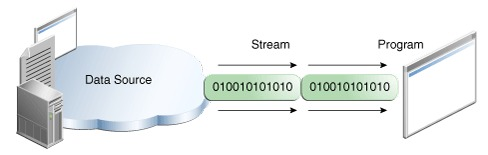
\includegraphics[scale=.45]{../img/java-io-ins}
\begin{flushright}
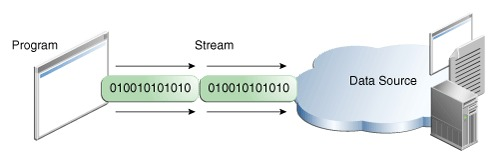
\includegraphics[scale=.45]{../img/java-io-ins2} 
\end{flushright}
\begin{center}
{\scriptsize Source Oracle}
\end{center}
\end{frame}

\begin{frame}{Les flux standards}
Lorsqu'un programme s'ex�cute, 3 flux existent automatiquement
  \begin{itemize}
  \item � priori connect�s au clavier et � l'�cran
  \item Mais peut �tre chang� via une <<redirection>>
  \\(cf. cours de syst�me et exercices Linux au laboratoire)
  \end{itemize}
\bigskip
\java|System.in| : l'entr�e standard
  \begin{itemize}
  \item De type \java|InputStream|
    \begin{itemize}
    \item Classe g�n�rale pour un flux binaire en entr�e
    \item \java|FileInputStream| h�rite de \java|InputStream|
    \end{itemize}
  \end{itemize}
\end{frame}

\begin{frame}{Les flux standards}
\java|System.out| : la sortie standard
  \begin{itemize}
  \item De type \java|PrintStream|
  \item Ce qui explique l'existence de \java|println|
  \end{itemize}
\bigskip
\java|System.err| : l'erreur standard
  \begin{itemize}
  \item Aussi de type \java|PrintStream|
  \item Flux s�par� ce qui permet de ne rediriger que les erreurs
  \end{itemize}
\bigskip
\emph{Exercice} : Expliquez la nature de chacun des �l�ments de 
\java|System.out.println("Hello");|
\end{frame}

\subsection{Donn�es primitives formatt�es}
\leconwithtocinside

\begin{frame}[fragile]{Donn�es primitives formatt�es}
Les textes ayant pour vocation d'�tre lus par des humains
  \begin{itemize}
  \item On veut un \emph{contr�le fin} sur la \emph{mise en page} des textes produits
  \item On doit �tre capable de \emph{g�rer} une \emph{mise en page complexe} du texte lu
  \end{itemize}
\end{frame}

\begin{frame}[fragile]{�criture de donn�es formatt�es}
\java|PrintWriter| offre �galement la m�thode \java|printf| 
  \begin{itemize}
  \item Permet un contr�le tr�s fin de la sortie
  \item \emph{Exemple}
    \begin{Java}
public void test(PrintStream out) {  // Un fichier, l'�cran, ...
  out.printf("%04d\n", 23);	                     // 0023
  out.printf("%4.2f\n", 12.2);	                  // 12.20

  Calendar c = GregorianCalendar.getInstance();
  c.set(9, 00, 23);                              // 23 janvier 2009
  out.printf("le %1$td/%1$tm/%1$ty\n", c);       // le 23/01/09
}
    \end{Java}
  \item cf. l'API pour tous les d�tails
\end{itemize}
\end{frame}

\begin{frame}[fragile]{Lecture de donn�es formatt�es}
Voyons � pr�sent toute la puissance de \java|Scanner|
  \begin{itemize}
  \item Seule classe vue ici qui n'est pas dans \java|java.io|
  \item Permet de d�composer une suite de caract�res
  \item Fonctionne sur
    \begin{itemize}
    \item Un \java|InputStream| (fichier binaire, entr�e standard, \dots)
    \item Mais aussi un \java|String|
    \\\emph{Exemple} : \java|new Scanner("3 14 15 92 65")|
    \end{itemize}
  \item L'entr�e est d�compos�e en \emph{tokens}
    \begin{itemize}
    \item Cf. le�on sur l'analyse lexicale 
    \item Le s�parateur est le \emph{whitespace} (configurable)
    \end{itemize}
  \end{itemize}
\end{frame}

\begin{frame}[fragile]{Lecture de donn�es formatt�es}
Fonctionnement de base
  \begin{itemize}
  \item � la cr�ation on est au d�but
  \item Chaque \java|next()| \emph{lit} un token
  \item \java{nextType} �quivaut � un \java|next| suivi d'une conversion en le bon 
       \textit{type} (pour certains types)
  \item \emph{Exemple}
     \begin{Java}
  Scanner uneEntr�e = new Scanner("12 true \n false");
  // \n est un whitespace aussi !
  int n = uneEntr�e.nextInt();
  boolean b = uneEntr�e.nextBoolean();
  String s = uneEntr�e.next();
    \end{Java}  
  \end{itemize}
\end{frame}

\begin{frame}[fragile]{Lecture de donn�es formatt�es}
Si l'entr�e ne correspond pas au type demand� :
  \begin{itemize}
  \item \java|InputMismatchException| est lanc�e
  \item Le token n'est pas \emph{consomm�}
  \item \emph{Exemple}
    \begin{Java}
  Scanner uneEntr�e = new Scanner("true 12");
  int n = 0;
  try {
    n = uneEntr�e.nextInt();
  } catch (InputMismatchException ex) {
    uneEntr�e.next(); // N�cessaire !
    n = uneEntr�e.nextInt(); 
  }
    \end{Java}
  \end{itemize}
\end{frame}

\begin{frame}[fragile]{Lecture de donn�es formatt�es}
\java|nextLine()| lit la chaine jusqu'� la fin de la ligne (lue mais non incluse)
  \begin{itemize}
  \item \emph{Exemple}
    \begin{Java}
  Scanner uneEntr�e = new Scanner("12 true \n false");
  String s = uneEntr�e.nextLine(); //"12 true "
    \end{Java}
  \item \emph{Exemple}
    \begin{Java}
  Scanner uneEntr�e = new Scanner("12\n suite");
  int n = uneEntr�e.nextInt();
  String s = uneEntr�e.nextLine(); // lit "" !!!
  s = uneEntr�e.nextLine(); // lit " suite" !!!
    \end{Java}
  \end{itemize}
\end{frame}

\begin{frame}[fragile]{Lecture de donn�es formatt�es}
Pas de \java|nextChar()|
  \begin{itemize}
  \item Peut �tre simul� par \java|next().charAt(0)|
  \item \emph{Exemple}
    \begin{Java}
  Scanner uneEntr�e = new Scanner("12 suite");
  char c1 = uneEntr�e.next().charAt(0); // 1
  char c2 = uneEntr�e.next().charAt(0); // s
    \end{Java}
  \end{itemize}
\end{frame}

\begin{frame}[fragile]{Lecture de donn�es formatt�es}
On peut imposer un \emph{sch�ma} de lecture
  \begin{itemize}
  \item via \java|next(String pattern)|
  \item La syntaxe est tr�s riche et un peu complexe (cf. les expressions
r�guli�res (\textit{regex}), classe Pattern dans la documentation). 
  \item \emph{Exemple} : le token doit �tre le caract�re "H", "h", "F" ou "f" sinon 
     \java|InputMismatchException|
    \begin{Java}
  String s = clavier.next("[HhFf]");
    \end{Java}
  \end{itemize}
\end{frame}

\begin{frame}[fragile]{Lecture de donn�es formatt�es}
\begin{itemize}
	\item \emph{Exemple} : lire un op�rateur : +, -, * ou /
	\begin{Java}
  String s = clavier.next("[\\+\\-\\*/]");
	\end{Java}

	\item \emph{Exemple} : lire un login �tudiant
	\begin{Java}
  String s = clavier.next("[gG]\\d{5}");
	\end{Java}

	\item \emph{Remarque} : on �chappe (via le caract�re $\backslash$ ) deux fois 
	certains caract�res afin de leur rendre leur sens premier (ils en ont deux)
	\begin{itemize}
		\item une fois � cause de "\java{String}",
		\item une deuxi�me fois � cause de la \textit{regex}
	\end{itemize}
\end{itemize}
\end{frame}

\begin{frame}[fragile]{Lecture de donn�es formatt�es}
Les m�thodes de la forme \java|hasNext()| permettent de savoir
  \begin{itemize}
  \item Si un token est disponible en entr�e
    \begin{Java}
  int somme = 0;
  while ( clavier.hasNextInt() ) {
      somme = somme + clavier.nextInt();
  }
    \end{Java}
  \item S'il est du bon type
    \begin{Java}
  System.out.println( "Je voudrais un entier" );
  while( !clavier.hasNextInt() ) {
      System.out.println( "Message d'erreur" );
      clavier.next(); // passer l'entr�e erron�e
  }
  int n = clavier.nextInt();
    \end{Java}
  \end{itemize}
\end{frame}

\begin{frame}[fragile]{Lecture de donn�es formatt�es}
La notion de <<locale>>
  \begin{itemize}
  \item Un \emph{locale} repr�sente les habitudes locales de l'utilisateur
  (ex: la \emph{virgule d�cimale} pour les francophones)
  \item Par d�faut un scanner prend le locale propre au syst�me
  \item On peut en d�terminer un autre
  \item Ex : nombres flottants � \emph{l'anglaise}
    \begin{Java}
  Scanner clavier = new Scanner(System.in); 
  clavier.useLocale(Locale.UK);
    \end{Java}
  \end{itemize}
\end{frame}

\begin{frame}[fragile]{La classe <<Console>>}
Avec un seul objet de type \java|Console|, il est possible de \emph{lire} et
\emph{�crire} ... dans la console
	\begin{itemize}
	\item obtenir une console
		\begin{Java}
		Console console = System.console();
		if (console == null) {
		    System.out.println("Sorry ...");
		    System.exit(1);
		}
		\end{Java}
	\item lecture 
		\begin{Java}
		String name = console.readLine("Enter name:");
		\end{Java}
	\end{itemize}
\end{frame}

\begin{frame}[fragile]{La classe <<Console>>}
	\begin{itemize}
	\item �criture format�e
		\begin{Java}
		console.format("Your name is %s", name);
		\end{Java}
	\item lire un mot de passe
		\begin{Java}
		char[] password = console.readPassword("Enter your password: ");
		// some work
		Arrays.fill(password, ' ');
		\end{Java}
	\end{itemize}
\end{frame}

\subsection{Lire/�crire des objets}
\leconwithtocinside

\begin{frame}{S�rialisation}
Nous savons � pr�sent lire/�crire des valeurs primitives
\\\bigskip
Quid des objets ?
  \begin{itemize}
  \item Revient � sauver tous les attributs
  \item Dont certains sont aussi des objets
  \item $\Longrightarrow$ plus complexe
  \item On s'en sort via la <<s�rialisation>>
  \end{itemize} 
\bigskip
\emph{S�rialiser} : Transformer un objet (ses attributs) en une suite d'octets
\end{frame}

\begin{frame}[fragile]{S�rialisation}
Pour l'�criture, on utilise \java|ObjectOutputStream|
  \begin{itemize}
  \item \emph{Exemple} : �criture d'objets
    \begin{Java}
  FileOutputStream out = new FileOutputStream("theTime");
  ObjectOutputStream s = new ObjectOutputStream(out);
  s.writeObject("Today");
  s.writeObject(new Date());
  s.close();
  out.close();
    \end{Java}
  \end{itemize}
\end{frame}

\begin{frame}[fragile]{S�rialisation}
Pour la lecture, on utilise \java|ObjectInputStream|
  \begin{itemize}
  \item \emph{Exemple} : Relecture des objets
\begin{Java}
  FileInputStream in = new FileInputStream("theTime");
  ObjectInputStream s = new ObjectInputStream(in);
  String today = (String) s.readObject();
  Date date = (Date) s.readObject();
  s.close();
  in.close();
\end{Java}
  \item � la lecture, le casting est n�cessaire car \java|readObject()| retourne un \java|Object|
\end{itemize}
\end{frame}

\begin{frame}[fragile]{S�rialisation}
Une classe doit impl�menter \java|Serializable| pour �tre s�rialisable 
  \begin{itemize}
  \item Pas de m�thode, sert juste de <<tag>>
  \item Tous ses attributs doivent aussi �tre s�rialisables
  \end{itemize}
\bigskip
\emph{Exemple}
\begin{itemize}
\item []
\begin{Java}
  public class MaClasse implements Serializable {...}
\end{Java}
\end{itemize}
\end{frame}

\begin{frame}{S�rialisation}
La s�rialisation est utilis�e pour
  \begin{itemize}
  \item La communicaton r�seau entre processus \sigle{Java}
  \item La sauvegarde des donn�es d'une application. Mais
    \begin{itemize}
    \item Pas tr�s efficace : tout est lu ou sauv� en bloc
    \item La classe ne doit pas avoir chang� entre le moment de l'�criture et le moment de la relecture $\Longrightarrow$ probl\`eme de p�rennit� de l'information
    \end{itemize}
  \end{itemize}
\end{frame}


\section{Les entr�es-sorties (NIO2)}
\leconwithtoc 

\subsection{Pr�sentation}
\leconwithtocinside

\begin{frame}[fragile]{Pr�sentation}
\emph{Pr�alable} Le \textit{package} NIO.2, comme pr�sent�, concerne le JDK 7 (et suivants)
\end{frame}

\subsection{Notion de <<varargs>>}
\leconwithtocinside 

\begin{frame}[fragile]{Notion de <<varargs>>}
\emph{Principe} \textit{varargs} est un principe java permettant 
d'�crire des m�thodes acceptant un nombre variable d'arguments

\bigskip Une m�me m�thode \texttt{foo} peut-�tre appel�e 
\begin{Java} 
foo("one");
foo("one","two");
String[] ss = {"one", "two", "three"};
foo(ss);
\end{Java} 

Pour ce faire, 
\begin{Java} 
public void foo(String... ss) { <enter code here> }
\end{Java} 

... et le param�tre re�u est un \textbf{simple tableau}
\end{frame}

\subsection{L'interface <<Path>>}
\leconwithtocinside 

\begin{frame}[fragile]{L'interface <<Path>>}
Un \emph{fichier} est identifi� par son chemin � travers le \textit{filesystem}, 
on parle aussi de 
	\begin{itemize}
		\item son nom compl�tement qualifi� (FQN - \textit{Fully Qualified Name}), 
		\item son \textit{\textbf{Path}} (qui signifie \textit{chemin})
	\end{itemize}
Par exemple 
	\begin{itemize}
		\item \texttt{/home/alice/java/Hello.java} ou 
		\item \verb|C:\Users\alice\java\Hello.java|
	\end{itemize}
\end{frame}

\begin{frame}[fragile]{L'interface <<Path>>}
Rappels
	\begin{itemize}
		\item le s�parateur (\textit{delimiter}) est diff�rent en fonction du \textit{filesystem}
		\item un chemin (\textit{path}) peut-�tre \textbf{relatif} ou \textbf{absolu}
		\item certains syst�mes de fichiers autorisent la notion de \textbf{lien symbolique} 
		(\textit{symbolic link})
	\end{itemize}
\end{frame}

\begin{frame}[fragile]{L'interface <<Path>>}
L'interface \emph{\texttt{Path}} en java repr�sente un 
chemin (\textit{path}) et permet de le manipuler
	\begin{itemize}
		\item cr�er un \textit{path}
		\item utiliser l'information contenue dans un \textit{path}
		\item convertir un \textit{path}
		\item comparer deux \textit{path}
		\item ...
	\end{itemize}
La classe \texttt{\emph{Paths}}
est une classe utilitaire permettant de cr�er un \textit{path} (une
\textit{Factory}) \\
\bigskip
\emph{Remarque}: Le fichier que le chemin repr�sente peut ne pas exister
\end{frame}

\begin{frame}[fragile]{L'interface <<Path>>}
\begin{itemize}
\item Cr�er un \textit{path}
	\begin{Java}
	Path path1 = Paths.get("/tmp/foo");
	Path path2 = Paths.get(System.getProperty("user.home"),
	    "logs", "foo.log");
	\end{Java} 
\item Utiliser les informations contenues dans un \textit{path} \\
{\small (Soit la d�claration (dans un contexte linux))}
		\begin{Java} 
		Path path = Paths.get("/home/alice/foo");
		\end{Java} 
		\begin{itemize}
			\item \texttt{toString} $\longrightarrow$ /home/alice/foo
			\item \texttt{getFileName} $\longrightarrow$ foo
			\item \texttt{getParent} $\longrightarrow$ /home/alice
			\item \texttt{getRoot} $\longrightarrow$ /
		\end{itemize}
\end{itemize}
\end{frame}

\begin{frame}[fragile]{L'interface <<Path>>}
\begin{itemize}
\item Convertir un \textit{path}
\begin{itemize}
\item \textbf{\texttt{toUri()}} \\ 
vers une uri (\textit{uniform resource identifier})
\begin{Java} 
Path path = Paths.get("/var/log/syslog");
System.out.println(path.toUri());
\end{Java} 
$\longrightarrow$ file:///var/log/syslog
\item \textbf{\texttt{toAbsolutePath()}} \\ 
vers un chemin absolu (si \texttt{pwd $\rightarrow$ /home/alice})
\begin{Java} 
Path path =  Paths.get("file");
System.out.println(path.toAbsolutePath());
\end{Java} 
$\longrightarrow$ /home/alice/file
\end{itemize}
\end{itemize}
\end{frame}

\begin{frame}[fragile]{L'interface <<Path>>}
\begin{itemize}
\item Convertir un \textit{path} (suite)
	\begin{itemize}
		\item \textbf{\texttt{toRealPath()}}  
		vers un chemin <<r�el>>
		\begin{itemize}
			\item \textit{idem} que \texttt{toAbsolutePath()} mais 
			\item si c'est un \textbf{lien}, il est remplac� par le chemin vers
			lequel le lien pointe
		\end{itemize}
		\item \begin{Java} 	
Path path = Paths.get(args[0]);
Path fqnPath = null;
// ...
fqnPath = path.toRealPath();
// ...
System.out.println("Old path: " + path);
System.out.println("New path: " + fqnPath);
		\end{Java} 
		{\small (extrait de la classe \texttt{RealPath.java})}
	\end{itemize}
\end{itemize}
\end{frame}

\begin{frame}[fragile]{L'interface <<Path>>}
\begin{itemize}
	\item Convertir un \textit{path} (suite)
	\begin{itemize}
		\item \textbf{\texttt{toRealPath}} (suite)
		\begin{itemize}
		\item Soit la situation suivante
		\begin{Java} 
$ls -l /elsewhere
-rw-r--r-- 1   bob bob  592 Jan 13 16:56 file
lrwxrwxrwx 1   bob bob  13 Jan 13 16:57 link -> file
		\end{Java} 
		\item \texttt{java RealPath file} $\longrightarrow$ /elsewhere/file
		\item \texttt{java RealPath /elsewhere/file} $\longrightarrow$ /eslewhere/file
		\item \texttt{java RealPath link} $\longrightarrow$ /elsewhere/file
		\end{itemize}
	\end{itemize}
\end{itemize}
\end{frame}

\begin{frame}[fragile]{L'interface <<Path>>}
\begin{itemize}
\item Convertir un \textit{path} (suite)
\begin{itemize}
\item \textbf{\texttt{resolve(Path)}} \\
permet de cr�er un chemin sur base de deux chemins incomplets
\begin{Java} 
Path path;
path = Paths.get(".").toRealPath();
System.err.println("Error: " + e.getMessage());
System.exit(1);
}
System.out.println("Path: " + path);		
System.out.println("Path: " + path.resolve("file"));			
\end{Java} 
\texttt{java ResolvePath} $\longrightarrow$  \\ 
    Path: /elsewhere \\ 
    Path: /elsewhere/file
\end{itemize}
\end{itemize}
\end{frame}

\begin{frame}[fragile]{L'interface <<Path>>}
\begin{itemize}
\item ... et finalement la classe \texttt{Path}
\begin{itemize}
\item impose une m�thode \texttt{equals(Object)}
\item ajoute des m�thodes
	\begin{itemize}
	\item \texttt{startWidth(Path)} et \texttt{startWidth(String)}
	\item \texttt{endsWidth(Path)} et \texttt{endsWidth(String)}
	\item \texttt{isSameFile()} (voir plus loin, la classe \texttt{Files})
	\end{itemize}
\item impl�mente \texttt{Iterable}
\item impl�mente \texttt{Comparable}
\end{itemize}
\end{itemize}
\end{frame}

\subsection{Op�rations sur les fichiers, la classe <<Files>>}
\leconwithtocinside 

\begin{frame}[fragile]{Op�rations sur les fichiers, la classe <<Files>>}
La classe \emph{\texttt{Files}} est la deuxi�me classe utilitaire importante du
\textit{package} NIO.2

V�rifier (\textit{checking}) un fichier ou un r�pertoire
	\begin{itemize}
	\item \textbf{\texttt{exists(Path, LinkOption\dots)}} teste l'existence
	\begin{Java} 
	Files.exists(path);
	Files.exists(path, LinkOption.NOFOLLOW_LINKS));
	\end{Java}
	\item \textbf{\texttt{notExists(Path, LinkOption\dots)}} teste la non-existence 
	\begin{Java} 
	Files.notExists(path);
	\end{Java} 
	\item Ces deux m�thodes ne sont pas compl�mentaires ... 
	\end{itemize}
\end{frame}

\begin{frame}[fragile]{Op�rations sur les fichiers, la classe <<Files>>}
V�rifier (\textit{checking}) un fichier ou un r�pertoire (suite)
\begin{itemize}
	\item \textbf{\texttt{isReadable(Path)}} v�rifie si le fichier est accessible en lecture
	\item \textbf{\texttt{isWritable(Path)}} v�rifie si le fichier est accessible en �criture
	\item \textbf{\texttt{isExecutable(Path)}} v�rifie si le fichier est accessible en ex�cution
	\item \textbf{\texttt{isSameFile(Path, Path)}} v�rifie si les deux chemins 
	renseignent le m�me fichier
\end{itemize}
\end{frame}

\begin{frame}[fragile]{Op�rations sur les fichiers, la classe <<Files>>}
Effacer (\textit{delete}) un fichier ou un r�pertoire vide
\begin{itemize}
	\item \textbf{\texttt{delete(Path)}} \\
	lance une exception si le fichier/r�pertoire n'existe pas
	\item \textbf{\texttt{deleteIfExists(Path)}}
\end{itemize}
\begin{Java} 
try {
    Files.delete(path);
} catch (NoSuchFileException x) {
    System.err.format("%s: no such" +
        " file or directory%n", path);
} catch (DirectoryNotEmptyException x) {
    System.err.format("%s not empty%n", path);
} catch (IOException x) {
    // File permission problems are caught here.
    System.err.println(x);
}
\end{Java} 
\end{frame}

\begin{frame}[fragile]{Op�rations sur les fichiers, la classe <<Files>>}
Copier un fichier ou un r�pertoire
	\begin{itemize}
		\item \textbf{\texttt{copy(Path, Path, CopyOption\dots)}}
		\begin{itemize}
		\item Sans \textit{replace existing}, la copie �choue si le fichier existe
		\item Copier un r�pertoire vers un autre ne copie que le r�pertoire
		\textbf{pas son contenu}
		\end{itemize}
		\item Copie de fichiers ou de r�pertoires
\begin{Java} 
Files.copy(source, target);
Files.copy(source, target, CopyOption.REPLACE_EXISTING);
\end{Java} 
		\item Il existe deux m�thodes permettant de copier de/vers un 
		\textbf{autre type de flux}
		\begin{itemize}
			\item \texttt{copy(InputStream, Path, CopyOption\dots)}
			\item \texttt{copy(Path, OutputStream)}
		\end{itemize}
	\end{itemize}
\end{frame}

\begin{frame}[fragile]{Op�rations sur les fichiers, la classe <<Files>>}
D�placer un fichier ou un r�pertoire
	\begin{itemize}
		\item \textbf{\texttt{move(Path, Path, CopyOption\dots)}}
		\begin{itemize}
			\item \textit{idem} \texttt{copy}
		\end{itemize}
	\end{itemize}
\end{frame}

\begin{frame}[fragile]{Op�rations sur les fichiers, la classe <<Files>>}
Obtenir les m�tadonn�es d'un fichier \\
(quelques m�thodes en vrac) \\ 
\begin{center}\tt
size(Path) isHidden(Path)  isDirectory(Path) isRegularFile(Path)
isSymbolicLink(Path) getLastModifiedTime(Path, LinkOption...)
setLastModifiedTime(Path, \textit{FileTime})  \\  getOwner(Path, LinkOption...)
\\ setOwner(Path, \textit{UserPrincipal}) ...
\end{center}
\end{frame}

\begin{frame}[fragile]{Op�rations sur les fichiers, la classe <<Files>>}
Obtenir les m�tadonn�es d'un fichier (suite)
	\begin{itemize}
		\item \texttt{FileTime} repr�sente un temps associ� � un fichier. 
		Par exemple, un \textit{timestamp} dans une heure
\begin{Java} 
FileTime ft = FileTime.fromMillis(
    System.currentTimeMillis() 
       + (1000*60*60));
\end{Java} 
		\item La valeur de \texttt{UserPrincipal} est obtenue gr�ce au 
		\textit{user lookup service} comme suit
\begin{Java} 
UserPrincipal owner = FileSystems.getDefault()
    .getUserPrincipalLookupService()
    .lookupPrincipalByName("alice");
\end{Java} 
		{\small La classe \emph{\texttt{FileSystems}} est une classe utilitaire de
		NIO.2}
	\end{itemize}
\end{frame}

\subsection{O� l'on reparle de lire / �crire des fichiers}
\leconwithtocinside 

\begin{frame}[fragile]{O� l'on reparle de lire / �crire des fichiers}
Lire un fichier
\begin{itemize}
\item \textbf{Rappel} Pour lire un fichier, on faisait:
\begin{Java} 
try {
    BufferedReader reader = new BufferedReader(
        new FileReader("input.txt"));
    // lire 
    reader.close();
catch (IOException x) {
    // G�rer les erreurs
   if (reader != null) {
      try {
          reader.close();
      } catch (IOException x2) {
           // Plus rien � faire
      }
   }
}
\end{Java} 
\end{itemize}
\end{frame}

\begin{frame}[fragile]{O� l'on reparle de lire / �crire des fichiers}
Lire un fichier (suite)
	\begin{itemize}
		\item La classe \texttt{\emph{Files}} propose une m�thode  \\ 
		\hspace{1cm}\texttt{newBufferedReader(Path, Charset)}
		\begin{itemize}
			\item plus efficace
			\item \texttt{Closeable}
		\end{itemize}
		\bigskip
		\item C'est une \textbf{bonne pratique d'utiliser le \textit{try-with-resources}} car alors le compilateur g�n�re automatiquement le code permettant de fermer (\textit{close}) lesdites ressources (celles qui sont \texttt{Closeable})
	\end{itemize}
\end{frame}

\begin{frame}[fragile]{O� l'on reparle de lire / �crire des fichiers}
Lire un fichier (suite)
\begin{Java} 
// ...
Charset charset = Charset.forName("UTF-8");
Path file = Paths.get(args[0]);
try (BufferedReader reader = Files.newBufferedReader(file, charset)){
    String line = null;
    while ((line = reader.readLine()) != null) {
        System.out.println(line);
    }
} catch (IOException x) {
    System.err.format("IOException: %s%n", x);
    System.exit(1);
}
\end{Java} 
\end{frame}

\begin{frame}[fragile]{O� l'on reparle de lire / �crire des fichiers}
�crire un fichier
\begin{itemize}
\item De m�me, la classe \texttt{\emph{Files}} propose une m�thode  \\ 
\hspace{1cm}\texttt{newBufferedWriter(Path, Charset)}
\end{itemize}
\begin{Java} 
// ...
Charset charset = Charset.forName("UTF-8");
Path file = Paths.get(args[0]);
String s = "Hello world\n";
try (BufferedWriter writer = Files.newBufferedWriter(file, charset)){
    writer.write(s, 0, s.length());
} catch (IOException x) {
    System.err.format("IOException: %s%n", x);
}
\end{Java} 
\end{frame}


\begin{frame}[fragile]{O� l'on reparle de lire / �crire des fichiers}
D'autres m�thodes encore de la classe \texttt{\emph{Files}}
	\begin{itemize}
		\item \texttt{newInputStream(Path, OpenOption...)} retournant un
		\texttt{InputStream}
		\item \texttt{newOutputStream(Path, OpenOption...)} retournant un
		\texttt{OutputStream}
	\end{itemize}
\end{frame}

\begin{frame}[fragile]{O� l'on reparle de lire / �crire des fichiers}
D'autres m�thodes encore de la classe \texttt{\emph{Files}} (suite)
	\begin{itemize}
		\item \texttt{createTempFile(String, String)} pour cr�er un \textbf{fichier temporaire}
\begin{Java} 
try {
    Path tempFile =
        Files.createTempFile(null, ".myapp");
    System.out.format("The temporary file" 
        + " has been created: %s%n", tempFile);
} catch (IOException x) {
    System.err.format("IOException: %s%n", x);
}
\end{Java} 
$\longrightarrow$ The temporary file has been created: /tmp/8614889884323775294.myapp
	\end{itemize}
\end{frame}

\subsection{D�terminer le MIME type d'un fichier}
\leconwithtocinside 

\begin{frame}[fragile]{D�terminer le MIME type d'un fichier}
D�terminer le MIME type d'un fichier
\begin{itemize}
\item \texttt{probeContentType(Path)} permet d'obtenir le MIME type d'un fichier
\end{itemize}
\begin{Java} 
// ...
try {			 
    path = Paths.get(args[0]).toRealPath();
    String mimetype = Files.probeContentType(path);
    System.out.format("%s mimetype is %s\n", 
        path.getFileName(), 
        mimetype);
} catch (IOException x) {
    System.err.println(x);
    System.exit(1);
}
\end{Java} 
\end{frame}

\subsection{Au sujet des exceptions}
\leconwithtocinside 

\begin{frame}[fragile]{Au sujet des exceptions}
\begin{itemize}
	\item La plupart des m�thodes retournent une \texttt{IOException}
	\begin{itemize}
		\item \texttt{java.io.Exception}
	\end{itemize}
	\bigskip
	\item La classe \texttt{\emph{FileSystemException}} est une 
	\texttt{IOException} offrant plus d'informations sur l'exception
	\begin{itemize}
		\item \texttt{java.nio.file.FileSystemException}
		\item \texttt{getReason}, \texttt{getFile}, \texttt{getMessage}, \texttt{getOtherFile}
	\end{itemize}
\end{itemize}
\end{frame}

\begin{frame}[fragile]{Au sujet des exceptions}
\begin{itemize}
	\item Il pourrait �tre int�ressant d'�crire (par exemple) ...
\begin{Java} 
try {			 
    // ...
} catch (FileSystemException x) {
    System.err.format("%s - %s - %s\n",  x.getFile(), 
        x.getReason(), x.getMessage());
    System.exit(1);
} catch (IOException x) {
    System.err.println(x);
    System.exit(1);
}
\end{Java} 
\end{itemize}
\end{frame}

\subsection{Concepts NIO.2 non abord�s}
\leconwithtocinside 

\begin{frame}[fragile]{Concepts NIO.2 non abord�s}
Concepts NIO.2 non abord�s
	\begin{itemize}
	\item L'acc�s non s�quentiel aux fichiers 
	\href{http://docs.oracle.com/javase/tutorial/essential/io/rafs.html}{[lien]}
	\item La gestion des r�pertoires; cr�ation, parcours, ....
	\href{http://docs.oracle.com/javase/tutorial/essential/io/dirs.html}{[lien]}
	\item L'utilisation des \textit{hard links} par rapport aux \textit{soft links}
	\item Parcours du syst�me de fichiers 
	\href{http://docs.oracle.com/javase/tutorial/essential/io/walk.html}{[lien]}
	\item Recherche de fichiers, utilisation de \textit{wildcards} ou d'expression r�guli�re (\textit{regex})
	\item Surveillance de r�pertoires
	\end{itemize}
\end{frame}


\include{chapitre-conversion}
\include{chapitre-enum}

\section*{Annexe}
\begin{frame}{Cr�dits}
Ce document a �t� produit avec les outils suivants
\begin{itemize}
\item Les distributions \sigle{\emph{Ubuntu}} et/ou \sigle{\emph{debian}} 
du syst�me d'exploitation \sigle{\emph{Linux}}
\item \sigle{\emph{LaTeX}} comme syst�me d'�dition
\item La classe \sigle{\emph{Beamer}} pour les transparents 
\item Les packages \sigle{\emph{listings}}, \sigle{\emph{fancyvrb}}, \dots
\item Les outils \sigle{\emph{make}}, \sigle{\emph{rubber}}, \sigle{\emph{pdfnup}}, \dots
\end{itemize}
\end{frame}

\end{document} 
 
